% !TeX program = xelatex
% Final submission: two frozen research cycles, no additional model selection.
\documentclass[10pt,a4paper,twocolumn]{article}
\usepackage{fontspec}
\IfFontExistsTF{Times New Roman}{\setmainfont{Times New Roman}}{\setmainfont{Libertinus Serif}}
\IfFontExistsTF{Arial}{\setsansfont{Arial}}{\setsansfont{DejaVu Sans}}
\IfFontExistsTF{Consolas}{\setmonofont{Consolas}}{\setmonofont{Latin Modern Mono}}
\usepackage[russian]{babel}
\usepackage[margin=18mm,top=19mm,bottom=19mm,footskip=9mm]{geometry}
\usepackage{amsmath,amssymb,booktabs,microtype,graphicx,xcolor,titlesec,fancyhdr,balance}
\usepackage[font=small,labelfont={bf,sf},labelsep=period]{caption}
\usepackage[colorlinks=true,linkcolor=black,urlcolor=teal,citecolor=teal]{hyperref}
\definecolor{ink}{HTML}{243747}\definecolor{teal}{HTML}{167889}\definecolor{muted}{HTML}{657785}
\setlength{\columnsep}{7mm}\setlength{\parindent}{.8em}\setlength{\parskip}{1.5pt}
\setlength{\headheight}{14pt}\setlength{\textfloatsep}{9pt}\setlength{\dbltextfloatsep}{10pt}
\emergencystretch=2em\clubpenalty=10000\widowpenalty=10000\displaywidowpenalty=10000
\setcounter{dbltopnumber}{1}
\titleformat{\section}{\sffamily\bfseries\fontsize{11}{13}\selectfont\color{ink}}{\thesection}{.6em}{}
\titlespacing*{\section}{0pt}{9pt}{4pt}
\titleformat{\subsection}{\sffamily\bfseries\fontsize{9.5}{11.5}\selectfont}{\thesubsection}{.5em}{}
\titlespacing*{\subsection}{0pt}{6pt}{3pt}
\pagestyle{fancy}\fancyhf{}
\fancyhead[L]{\sffamily\fontsize{7}{8}\selectfont\color{muted}RL В ПОСЛЕДОВАТЕЛЬНЫХ РЕКОМЕНДАЦИЯХ}
\fancyhead[R]{\sffamily\fontsize{7}{8}\selectfont\color{muted}YAMBDA / GPT-2 / ИТОГОВАЯ РАБОТА}
\fancyfoot[C]{\sffamily\small\thepage}\renewcommand{\headrulewidth}{.25pt}\raggedbottom
\newcommand{\AUsers}{266}
\newcommand{\AQueries}{2770}
\newcommand{\ADelta}{-0.000037}
\newcommand{\ALo}{-0.000571}
\newcommand{\AHi}{+0.000497}
\newcommand{\BUsers}{637}
\newcommand{\BQueries}{6393}
\newcommand{\BDelta}{-0.000096}
\newcommand{\BLo}{-0.000162}
\newcommand{\BHi}{-0.000037}
\newcommand{\Gain}{28.5}

\begin{document}
\twocolumn[{
\begin{center}
{\sffamily\bfseries\fontsize{19}{22}\selectfont\color{ink}Оптимизация выученной награды\\в последовательных рекомендациях\par}
\vspace{5pt}
{\sffamily\fontsize{10}{12}\selectfont GPT-2, пятишаговый REINFORCE и проверка более сильной модели отклика\par}
\vspace{5pt}
{\sffamily\fontsize{8}{10}\selectfont\color{muted}Итоговая работа по задаче 2 / Yambda 50M / Октябрь 2026\par}
\end{center}
\vspace{3pt}
\noindent\textbf{Аннотация.} Исследуем, улучшает ли RL последовательные рекомендации,
если награду задаёт обученная модель отклика. В первом цикле обучены GPT-2,
четыре нейронные reward model и варианты REINFORCE с пятью наградами.
На \AUsers{} активных пользователях рост предсказанной награды не дал
подтверждённого прироста NDCG. Штраф за вымышленную историю также не помог:
$\Delta=\ADelta$, 95\% user-cluster CI $[\ALo;\AHi]$.
Во втором цикле усилили модель отклика и supervised baseline, затем
зарезервировали другую когорту. На \BUsers{} активных пользователях
copy-адаптер с CE повысил NDCG на \Gain\% относительно frozen GPT-2;
MSE новой reward model составила 0{,}0598 против 0{,}1844 у прежней сети на тех
же запросах. Тем не менее joint CE+reward с допуском по согласию моделей
уступил продолжению CE: $\Delta=\BDelta$, CI $[\BLo;\BHi]$.
Объясняем различие между точностью прогноза отклика и полезностью
градиента для выбора действия. Обе когорты относятся к одному периоду;
это не независимая репликация на будущей неделе.
\vspace{9pt}
}]

\section{Задача и исследовательский вклад}

Последовательная модель учится предсказывать следующий трек в логе.
RL позволяет сменить цель, например на долю прослушивания или дальнейшую
активность. Но отклик на новый выбор неизвестен: оптимизатор может
улучшать прогноз reward model (RM), используя её ошибки.
При генерации нескольких треков возникает ещё одна проблема:
рекомендация добавляется в историю, хотя пользователь мог её не слушать.

Проверены две конкретные идеи. Первая штрафует изменение RM между
реальной и дополненной историей. Вторая допускает reward-обновление,
только когда три RM согласны о направлении предпочтения между ветвями
генерации и копирования. Обе идеи получили отрицательный основной
результат. Отдельно получены улучшенный supervised baseline и существенно
более точная RM; их вклад не приписывается RL.

Работы о GPTRec~\cite{gptrec} и session-level REINFORCE~\cite{session}
показывают, как переносить RL в рекомендации. Мы не воспроизводим их
промышленный масштаб, off-policy correction или online-эффект.
Ансамбли RM~\cite{ensemble}, copy-механизмы~\cite{pointer,repeat} и
совместный NLL+RL~\cite{ada} --- известные подходы. Наш вклад состоит
в двух явно заданных модификациях, их контролируемой проверке и
анализе неудачи. Заявления мирового приоритета или общей гарантии нет.

\begin{figure*}[t]
\centering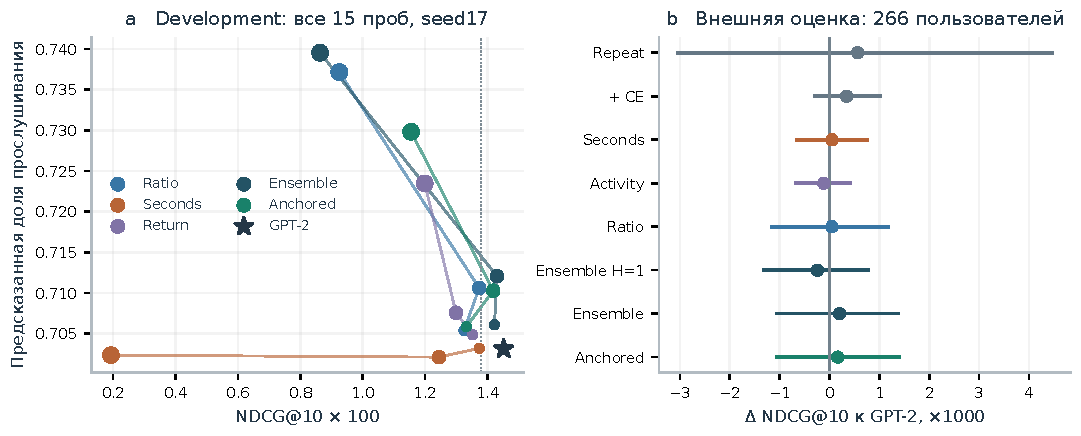
\includegraphics[width=.98\textwidth]{figures/cycle_a_search.pdf}
\caption{Цикл A: полный development search и внешние разности с GPT-2.
Вертикальная ось search показывает ratio RM также для других rewards;
размер точки растёт при уменьшении KL-штрафа;
пунктир --- правило 95\% SFT. У выбранных RL-вариантов CI к SFT включают 0.
Development используется для выбора, а не как подтверждающий результат.}
\label{fig:a}
\end{figure*}

\begin{figure*}[t]
\centering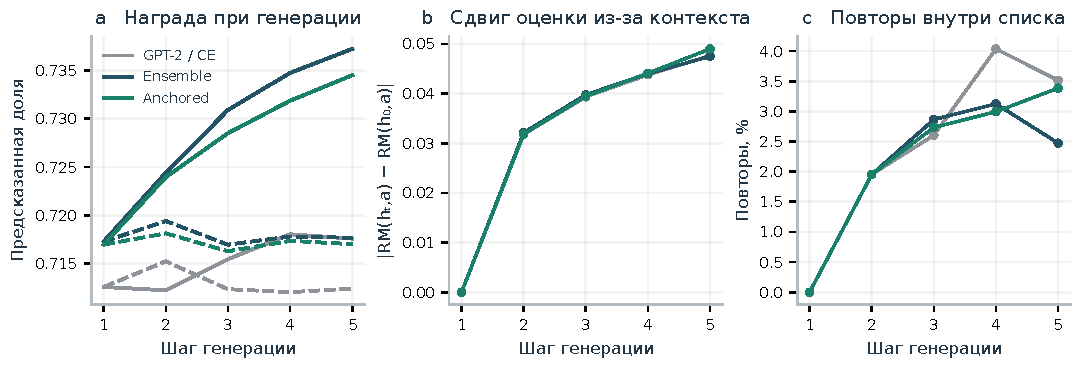
\includegraphics[width=.98\textwidth]{figures/cycle_a_rollouts.pdf}
\caption{Цикл A: связанные по RNG пятишаговые rollouts 256 пользователей.
Сплошные линии --- дополнение истории; пунктир в панели a ---
замороженная история. Собственные рекомендации повышают RM сильнее
при обновлении контекста. Это описательный аудит, не simulator oracle.}
\label{fig:rollout}
\end{figure*}

\begin{figure*}[t]
\centering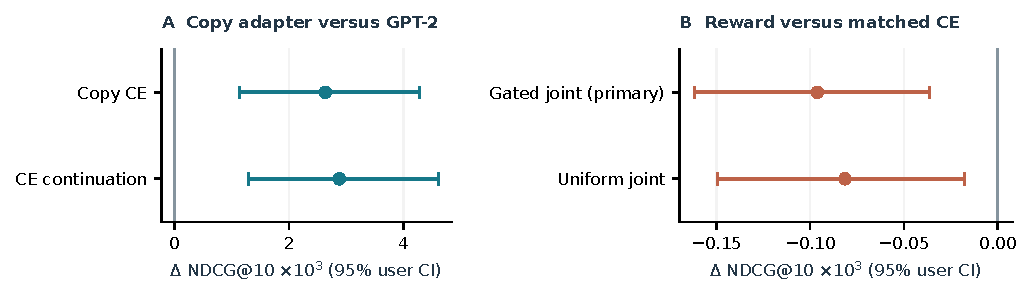
\includegraphics[width=.98\textwidth]{figures/cycle_b_effects.pdf}
\caption{Test B: улучшение supervised baseline и эффект reward разделены.
Слева --- copy против GPT-2; справа --- reward против matched CE.
Масштабы осей различаются. Primary --- gated joint. Интервалы контрольных
сравнений описательные. Точки A и B не объединяются в одну статистическую проверку.}
\label{fig:b}
\end{figure*}

\begin{figure*}[t]
\centering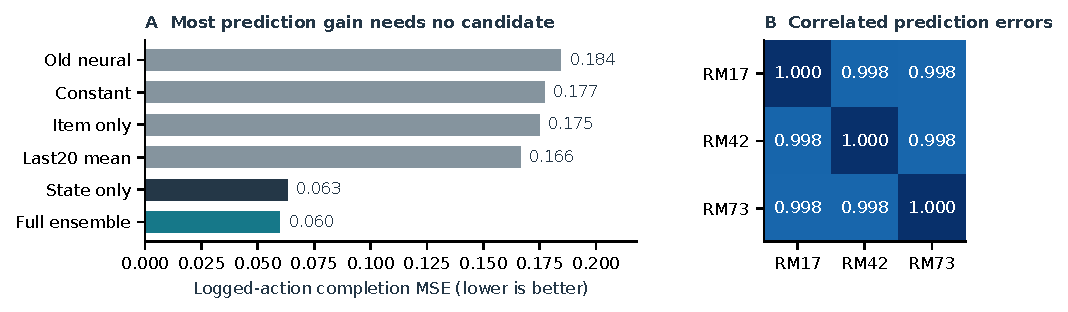
\includegraphics[width=.98\textwidth]{figures/cycle_b_reward.pdf}
\caption{Test B: старая и новая RM оценены на одних logged actions.
State-only --- одна модель, full --- ансамбль трёх; это не идеально
уравненная абляция ансамблей. Справа --- корреляция ошибок full RM.
Согласие близких моделей не является независимым свидетельством правильности.}
\label{fig:rm}
\end{figure*}

\section{Данные и протокол оценки}

Использована pinned таблица \texttt{listens} Yambda flat/50m:
46\,467\,212 строк,9238 UID, revision
\texttt{dd6f3a19eef5\ldots}. Поля: пользователь, item, timestamp,
organic flag, доля прослушивания и длительность. Время анонимизировано,
сутки равны 86\,400 секундам. Выбираются пользователи, сохраняются
\emph{все} исходные строки их историй.

\textbf{Цикл A.} После исключения UID прежних исследований выбраны 1200
пользователей, seed 718281; сохранены 5\,736\,029 строк.
Независимая перестановка делит UID на development 800 и external 400.
Обучение --- до day 270; search --- days 280--286 только development UID;
test --- days 293--298 только external UID. Ранние истории external UID
участвуют в train; их поздние метки не выбирают настройки.
Получены~\AQueries{} запросов \AUsers{} активных пользователей.

\textbf{Цикл B.} После открытия A исправлялись выявленные ограничения
на прежнем development. До новых fits выделены 1000 других UID,
seed 161803, не пересекающихся с A и прежними когортами; сохранены
5\,130\,518 строк. Эти UID целиком исключены из обучения.
Test-период тот же; получены~\BQueries{} запросов \BUsers{} активных
пользователей. Новая user-когорта даёт внешнюю проверку настроек,
но не заменяет проверку на другом периоде или сервисе.

Запрос --- первые до 4 неорганических событий с уникальным timestamp
за user-day. Нет отбора по completion. История строго раньше запроса;
одновременные события не образуют искусственно упорядоченных transitions.
Это оценка next logged listen, а не всех показов или удовлетворённости.

Для каждого сравнения методы имеют общий train-only каталог и одинаковые
запросы. Будущий target не добавляется в кандидаты. В A каталог ---
16\,384 частых трека;47{,}4\% целей вне словаря остаются промахами.
В B общий каталог --- 270\,376 исторических items; он покрывает 80{,}7\%
целей, head GPT-2 --- 48{,}6\%, достижимая поддержка head+copy --- 49{,}9\%.
Остальные цели тоже дают 0. Отдельный список misses не удаляется.

NDCG/Recall/MAP@10 для одного target сначала усредняются по model seeds
17/42/73, затем по запросам пользователя и пользователям. Для разностей
используется парный bootstrap 3000 user clusters. RM MSE усредняется
по событиям; resampling сохраняет кластеры и event weighting.
Основной контраст в каждом цикле зафиксирован до его test. Остальные
интервалы описательные, без заявления контроля семейной ошибки.
CI условны на данных и fits и не покрывают полный риск обучения.

\section{GPT-2 и пятишаговая RL-донастройка}

GPT-2 обучается с нуля на item IDs: learned token/position embeddings,
3 pre-LN causal blocks, width 128{,}4 heads, GELU, MLP expansion4,
final LayerNorm и tied input/output weights;2{,}70млн параметров.
Контекст 64, полная softmax по head-каталогу, редкие ID --- UNK.
Текстовые pretrained weights не используются.

AdamW: lr$=3\cdot10^{-4}$, decay 0{,}01, batch 64, warmup 300 и cosine.
Пилот 1500 updates дал слабый baseline; до test бюджет увеличен до 12\,000.
На development выбран checkpoint 3000, NDCG 0{,}01453; дальнейшее снижение
train CE не улучшило ranking. Поправка и полная траектория опубликованы.
Seeds 42/73 наследуют выбранное число updates. Контроли: popularity,
repeat, сглаженный Markov и ещё 120 updates CE.

Нейронная RM имеет отдельные item embeddings, mean/last history pooling,
взаимодействие с кандидатом и MLP с train-only длительностью.
Два sigmoid head предсказывают completion
$y=\operatorname{clip}(\texttt{played\_ratio\_pct}/100{,}0{,}1)$
и событие в $[t+1h,t+24h)$. Последнее называем Activity:
оно включает продолжающееся потребление, а не только возврат после ухода.
RM обучается на 855\,792 реально наблюдавшихся nonorganic actions до day 269,
чтобы label horizon заканчивался внутри train;800 updates, batch 512,
lr$10^{-3}$, BCE. Непрослушанные кандидаты не получают фиктивный нулевой reward.
Три seeds образуют ансамбль; четвёртая audit RM не оптимизируется, но
при тех же данных и архитектуре не является oracle.



\subsection{Награды и контроль вымышленной истории}
Пусть $m$ и $s$ --- среднее и population std ratio трёх RM.
Проверены Ratio (одна RM), Seconds
($\hat y\min(d,600)/600$), Activity ($0{,}5\hat y+0{,}5\hat p_{24}$),
Ensemble и предложенный Anchored:
\begin{align}
r_E(h_t,a)&=m(h_t,a)-0{,}5s(h_t,a),\\
r_A(h_t,a)&=r_E(h_t,a)-|m(h_t,a)-m(h_0,a)|.
\end{align}
Начальная $h_0$ реальна, $h_t$ содержит собственные generated IDs.
Anchored не позволяет бесплатно получить весь рост RM только за счёт
смены контекста. Он может подавлять полезную адаптацию; std ансамбля
не считается калиброванной неопределённостью.

REINFORCE работает on-policy в выученном surrogate, не в сервисе.
Из реального train prefix сэмплируются 5 действий; после каждого ID
добавляется в контекст без выдуманного playback outcome.
С frozen SFT $\pi_0$ определены
\begin{align}
\widetilde r_t&=r_t-\beta\log\frac{\pi_\theta(a_t|h_t)}{\pi_0(a_t|h_t)},\\
G_t&=\sum_{j=t}^{H-1}\gamma^{j-t}\widetilde r_j.
\end{align}
Градиент использует $\gamma^t(G_t-b_t)\nabla\log\pi_\theta$;
$b_t$ --- средний return остальных независимых trajectories batch.
Actor dropout выключен; lr$5\cdot10^{-5}$, $\gamma=0{,}9$,
batch 96{,}120 updates, grad clip 1.

На search проверены 15 точек:5 rewards и
$\beta\in\{0{,}02;0{,}1;0{,}5\}$. В семье выбирается максимальная predicted ratio
при NDCG не ниже 95\% SFT. Это правило отбора, не non-inferiority test.
Выбраны$\beta=0{,}1$ для Ratio/Ensemble/Anchored и 0{,}5 для Seconds/Activity.
Primary A --- Anchored$-$Ensemble при одинаковом$\beta=0{,}1$ и H5.
H1-контроль имеет те же updates, но меньше sampled actions.

\subsection{Результат A и поведение на пяти шагах}
\begin{table}[t]
\centering\small\setlength{\tabcolsep}{3pt}
\caption{Внешний test A: \AUsers{} активных UID, \AQueries{} запросов.
Это среднее трёх отдельных policy fits, не ансамбль политик.}
\begin{tabular}{lrrr}\toprule
Метод & NDCG@10 & Recall@10 & MAP@10\\\midrule
Popularity & 0.001982 & 0.004858 & 0.001112 \\
Markov & 0.006382 & 0.011533 & 0.004849 \\
Repeat & 0.011533 & 0.018675 & 0.009383 \\
GPT-2 & 0.010967 & 0.021340 & 0.007943 \\
+ CE & 0.011309 & 0.021894 & 0.008201 \\
Ratio & 0.011015 & 0.020923 & 0.008073 \\
Seconds & 0.011017 & 0.021537 & 0.007967 \\
Activity & 0.010853 & 0.020633 & 0.007971 \\
Ensemble H1 & 0.010722 & 0.021151 & 0.007666 \\
Ensemble H5 & 0.011169 & 0.021670 & 0.008038 \\
Anchored H5 & 0.011132 & 0.020675 & 0.008280 \\
\bottomrule\end{tabular}
\label{tab:a}
\end{table}

Ensemble повысил top1 proxy completion с 0{,}7143 до 0{,}7242,
но NDCG улучшилась лишь на 0{,}000202, CI$[-0{,}001047;0{,}001380]$.
Primary Anchored$-$Ensemble: \ADelta{}, CI$[\ALo;\AHi]$.
Ни выигрыш контекстного штрафа, ни прирост выбранных RL к SFT не подтверждены.

На development Seconds при слабом KL($\beta=0{,}02$) увеличил
длительность до 390с и занял одним треком 51{,}3\% top1;
NDCG упала до 0{,}00193. По правилу такая точка не выбрана.
У выбранных test-политик доминирующий top1 занимает около 1--2\% запросов.
Ratio сократил длительность с 192 до 182с, Seconds увеличил её примерно до 199с.
Награда меняет состав выдачи, но сама по себе не гарантирует релевантность.

RM A слаба: ratio MSE ансамбля 0{,}1798 против 0{,}1806 у константы,
надёжный выигрыш не установлен. Замена истории чужим ранее доступным
prefix повышает MSE до 0{,}2056. Activity AUC 0{,}568, Brier 0{,}1379 хуже
константы 0{,}1359. Сигнал активности не подтверждает улучшение retention.



В coupled rollout первый action совпадает при evolving/frozen history.
У Ensemble средняя proxy растёт примерно 0{,}717$\to$0{,}737 при дополнении
истории и остаётся около 0{,}718 на шаге 5 при замороженной истории.
Anchored не устранил сдвиг (рис.\ref{fig:rollout}). Реальных отзывов на
эти новые действия нет. На teacher-forced реальных продолжениях ошибка
RM выше; сравнение зависит и от отбора первых запросов и доступных шагов.

\section{Второй цикл: усиление baseline и RM}

Открытый test A больше не используется для выбора настроек.
Разрабатываем B на прежнем development, затем один раз открываем
другую заранее выделенную когорту. Frozen decoder и его 3 seeds сохраняются.

\subsection{Обучаемая смесь с историей}
Для head-распределения GPT-2 $p_0$ вводится
\begin{equation}
p_\theta(a|h)=(1-g_\theta(h))p_0(a|h)
+g_\theta(h)\sum_{j:h_j=a}c_\theta(j|h).
\end{equation}
Gate --- sigmoid от 13 признаков реального prefix и bias.
Copy softmax имеет recency decay и вес прошлого completion.
Масса повторных позиций суммируется. Обучаются 16 параметров адаптера,
а не весь transformer. Tail вне последних 64 событий недостижим:
расширение поддержки ограничено и не решает весь OOV.

CE-адаптер: до 40 случайных train contexts/user из days 240--269,
batch 256, Adam lr0{,}01, checkpoint 300/600/1200 выбирается на development
seed 17. Выбраны 1200 updates; другие seeds наследуют этот бюджет.
Fixed смесь 50/50 и repeat с head/full каталогом --- отдельные контроли.

\subsection{Более точная RM и допуск reward}
Новая RM --- ансамбль 3 CatBoostRegressor:13 признаков состояния
(прошлые completion, пропуски, длина истории, время) и 7 признаков
кандидата (статистики item, длительность, повтор и давность).
Item aggregates фиксируются до day 200; train --- days 200--259,
calibration --- 260--269. До 150/30 примеров на UID; сырая история сохранена.
Из глубин 4/6 и до 400 деревьев выбрана глубина 6 только по calibration MSE.
Past outcomes считаются доступными по timestamp лога; задержки неизвестны.

От CE адаптера все методы получают 300 updates, lr0{,}003:
\begin{equation}
\mathcal L=\mathcal L_{CE}+0{,}1D_{KL}(q_\theta\Vert q_{CE})
-\lambda I(h)\widehat{\mathbb E}_{p_\theta}[r].
\end{equation}
$q$ --- branch/position distribution; его KL ограничивает сверху KL
marginal item policy. CE continuation имеет$\lambda=0$;
reward-only убирает CE, сохраняя KL; uniform joint имеет$I=1$.
Gated допускает reward, если все RM согласны о знаке
$\mathbb E_c[r]-\mathbb E_{p_0}[r]$. Критерий не читает logged target.
Ожидание по copy точное, по frozen head --- 8 MC samples/context.
Для этой конечной смеси градиент reward доступен напрямую:
это H1 contextual-bandit адаптация, не full-decoder H5 REINFORCE.

Проверены 12 reward trials seed 17,
$\lambda\in\{0{,}1;0{,}5;2;8\}$ для трёх семейств.
Выбор --- максимальный search NDCG среди точек с proxy не ниже CE;
выбраны 0{,}1 для reward-only и 2 для joint/gated. Primary B --- gated$-$CE
continuation с одинаковым дополнительным бюджетом.
В AdaGRPO~\cite{ada} допуск зависит от рангов target/distractors;
наш target-free критерий не является воспроизведением этого алгоритма.



\section{Проверка на новой когорте}
\begin{table}[t]
\centering\small\setlength{\tabcolsep}{3pt}
\caption{Внешний test B: \BUsers{} активных UID, \BQueries{} запросов.
Сравнивать абсолютные значения между таблицами A/B как эффект метода нельзя.}
\begin{tabular}{lrrr}\toprule
Метод & NDCG@10 & Recall@10 & MAP@10\\\midrule
Popularity & 0.003370 & 0.007510 & 0.002099 \\
Repeat / head & 0.008787 & 0.014725 & 0.006964 \\
Repeat / full & 0.011983 & 0.020471 & 0.009352 \\
GPT-2 & 0.010095 & 0.020913 & 0.006888 \\
Copy 50/50 & 0.011837 & 0.020592 & 0.009148 \\
Copy CE & 0.012731 & 0.025023 & 0.009081 \\
CE continuation & 0.012977 & 0.025332 & 0.009291 \\
Reward-only & 0.012718 & 0.025030 & 0.009063 \\
Joint & 0.012895 & 0.025307 & 0.009199 \\
Gated joint & 0.012880 & 0.025267 & 0.009192 \\
\bottomrule\end{tabular}
\label{tab:b}
\end{table}

CE continuation получил 0{,}012977 против 0{,}010095 у GPT-2:
+\Gain\%, абсолютный прирост 0{,}002882,
CI$[0{,}001290;0{,}004613]$. Copy CE до продолжения --- 0{,}012731.
Превосходство над repeat не установлено: разность 0{,}000994,
CI$[-0{,}001616;0{,}003283]$. Поэтому результат не объявляется победой
над всеми сильными простыми методами.

Primary B отрицателен: gated$-$CE \BDelta{}, CI$[\BLo;\BHi]$,
около$-0{,}74\%$. Снижение мало, но интервал исключает 0.
Uniform joint также немного уступает CE: $-0{,}000081$,
CI$[-0{,}000150;-0{,}000018]$. Gated пропускает 88{,}5\% train contexts
и мало отличается от uniform. Proxy top1 при этом растёт
с 0{,}618404 до 0{,}618582; это прогноз, не измеренный эффект рекомендации.



На тех же запросах B старая neural RM имеет MSE 0{,}184392,
новая --- 0{,}059784, константа --- 0{,}176966. Снижение относительно
константы 66{,}2\%; CI разности$[-0{,}124936;-0{,}109805]$.
Но state-only RM, вообще без кандидата, уже имеет MSE 0{,}063096:
она даёт примерно 97\% сокращения MSE полного ансамбля относительно константы.
Full лучше: CI разности$[-0{,}004046;-0{,}002591]$, при различии бюджета.
Одна full RM seed 17 также сильна, MSE 0{,}059975.
Ошибки трёх full RM коррелируют около 0{,}998 (рис.\ref{fig:rm}).

Предсказуемость состояния пользователя даёт низкую общую MSE, но не
обязательно полезное различие между действиями. Это согласуется с
риском reward overoptimization~\cite{overopt}, хотя не доказывает
единственную причину снижения NDCG. Новая RM использует более богатую
информацию: её сравнение со старой сетью не изолирует архитектуру.
Popularity имеет proxy 0{,}648050 при NDCG 0{,}003370: максимум RM и next-item
релевантность явно расходятся.

В описательном post-test аудите длительность top1 пересчитана по
метаданным, известным к train cutoff 270: CE189{,}2с, gated189{,}1с.
Ранний duration200 кэш имел unknown=0 (13{,}2\% top1 CE в user-macro),
что занижало среднее. Исходный кэш сохранён; policy, reward и первичные
метрики не менялись.

\section{Воспроизводимость и выводы}

Код проверяет сохранение всех исходных строк выбранных UID, отсутствие
пересечений когорт, временные границы и неизменность входов при замене
будущего. В A выполнен точный replay24 neural top10 forecasts.
В обоих циклах forecasts запечатаны до labels. Компактные evidence
содержат raw top10, per-user/query метрики, все seeds/trials, RM predictions,
rollouts и цепочку SHA. Проверка без датасетов/GPU заново считает числа,
а не только сверяет готовый JSON. Тест подмены NDCG при обновлённом
checksum отвергается.

Цикл A:48 завершённых fits с пилотом,573с суммарных записанных fit stages;
CUDA peak 589{,}5MiB, max RSS \emph{на конец fit}1656MiB, не peak RSS.
Цикл B:24 fits адаптера,4 RM search fits и 2 диагностические RM;
записано 30{,}5с адаптеров,27{,}2с кэшей и 6{,}3с основного RM поиска.
Оборудование: i7-14700KF,48GB RAM, RTX4070TiSUPER16GB.
Это измерения отдельных этапов, не полный wall time исследования:
подготовка, сбои, часть диагностик и ручная работа не включены.
B переиспользует три SFT, поэтому его числа не показывают цену обучения
политики с нуля. Полные журналы сохраняют также неудачные варианты.

Ограничения: один сервис и период, ограниченная поддержка каталога,
короткий контекст, неизвестные задержки outcomes и небольшой бюджет HPO.
Модели B не обучались на новых UID, но их реальная история доступна
в момент запроса. Нельзя переносить эффект 16-параметрического H1 адаптера
на full-decoder H5 RL. Нет propensities, контрфактуальных labels,
IPS/DR оценки или online A/B. Activity не измеряет causal retention,
completion не равен удовлетворённости. Все tests теперь открыты;
следующий подтверждающий вывод требует новой внешней проверки.

\textbf{Вывод.} Усиление supervised policy и модели отклика дало
воспроизводимый прирост соответствующих метрик. Ни штраф за вымышленную
историю, ни допуск по согласию RM не подтвердили пользу RL;
во втором случае измерено небольшое ухудшение. Для следующих работ
недостаточно уменьшать общую MSE: нужно проверять способность RM
различать действия и независимость ошибок, а качество рекомендаций
подтверждать отдельно от proxy reward.

\vspace{3pt}
\noindent\textbf{Материалы.}\par
{\footnotesize\raggedright\noindent
Главный файл: \texttt{article.pdf}. Исходник:\par
\nolinkurl{code/paper/submission_task2/article.tex}.\par
Результаты: \nolinkurl{code/reports/task2/},
\nolinkurl{code/reports/task2b/}.\par
Из \texttt{code/}: \texttt{uv sync --locked --extra dev}, затем\par
\texttt{uv run --locked python scripts/verify\_submission.py}.\par}

\balance
\begin{thebibliography}{9}\small\setlength{\itemsep}{1pt}
\bibitem{gptrec} Petrov, Macdonald. Aligning GPTRec with Beyond-Accuracy Goals
with Reinforcement Learning. 2024. \href{https://arxiv.org/abs/2403.04875}{arXiv:2403.04875}.
\bibitem{session} Matveev et al. Session-Level Optimization for Large-Scale
Retrieval using REINFORCE with Multi-Step Off-Policy Correction. 2026.
\href{https://arxiv.org/abs/2607.02818v2}{arXiv:2607.02818v2}.
\bibitem{ensemble} Coste et al. Reward Model Ensembles Help Mitigate
Overoptimization. ICLR 2024. \href{https://arxiv.org/abs/2310.02743}{arXiv:2310.02743}.
\bibitem{pointer} Merity et al. Pointer Sentinel Mixture Models. ICLR 2017.
\href{https://arxiv.org/abs/1609.07843}{arXiv:1609.07843}.
\bibitem{repeat} Ren et al. RepeatNet: A Repeat Aware Neural Recommendation
Machine for Session-based Recommendation. AAAI 2019.
\href{https://arxiv.org/abs/1812.02646}{arXiv:1812.02646}.
\bibitem{ada} Xu et al. Adaptive Loss Balancing for Noise-Robust GRPO in
Generative Recommendation. Препринт 2026.
\href{https://arxiv.org/abs/2606.08480}{arXiv:2606.08480}.
\bibitem{overopt} Gao, Schulman, Hilton. Scaling Laws for Reward Model
Overoptimization. 2022. \href{https://arxiv.org/abs/2210.10760}{arXiv:2210.10760}.
\end{thebibliography}
\end{document}
